\subsection{Hardware}
   This section includes a list of all the hardware we have been (very generously) lent and have been working with for the duration of this project. The following list and images should be able to supply a better understanding and familiarization of the project.\\
	\\Cameras (figure 1):  
    		\begin{itemize}
		\item GS3-U3-41C6NIR-C (PointGrey/GrassHopper)
		\item GS3-U3-41C6C-C
		\item GS3-U3-23S6C-C\\
		\end{itemize}
	Lenses (figure 1): 
		\begin{itemize}
		\item EVS-3000 (figure 6)
		\item 2 x LS-TP-08 (Standard) (figure 7)\\
		\end{itemize}					
	Single Board Computers: 
		\begin{itemize}
		\item Jetson TK1 (figure 2) 
		\item Jetson TX1 developer kit with on-board camera (figure 3 and 4)\\
		\end{itemize}		
	Extras: 
		\begin{itemize}
		\item NIR Pass filter - blocks visible light while allowing NIR light through
		\item 2-port USB 3.0 supersede PCIe Card (figure 5)
		\item Camera mount
		\item 3 x USB 3.0 cables
		\item 1080p monitor (TV)\\
		\end{itemize}
		
\begin{figure}[!ht]
	  \centering
		    \includegraphics[width=0.6\textwidth,natwidth=610,natheight=642]{images/cameras.jpg}
		    \caption{The 3 PointGrey cameras provided by Rockwell Collins on a mount}
				\end{figure} 
 \begin{figure}[!ht]
	  \centering
		    \includegraphics[width=0.6\textwidth,natwidth=610,natheight=642]{images/JetsonTK1.jpg}
		      \caption{The Jetson TK1}
				\end{figure}
\begin{figure}[!ht]
	  \centering
		    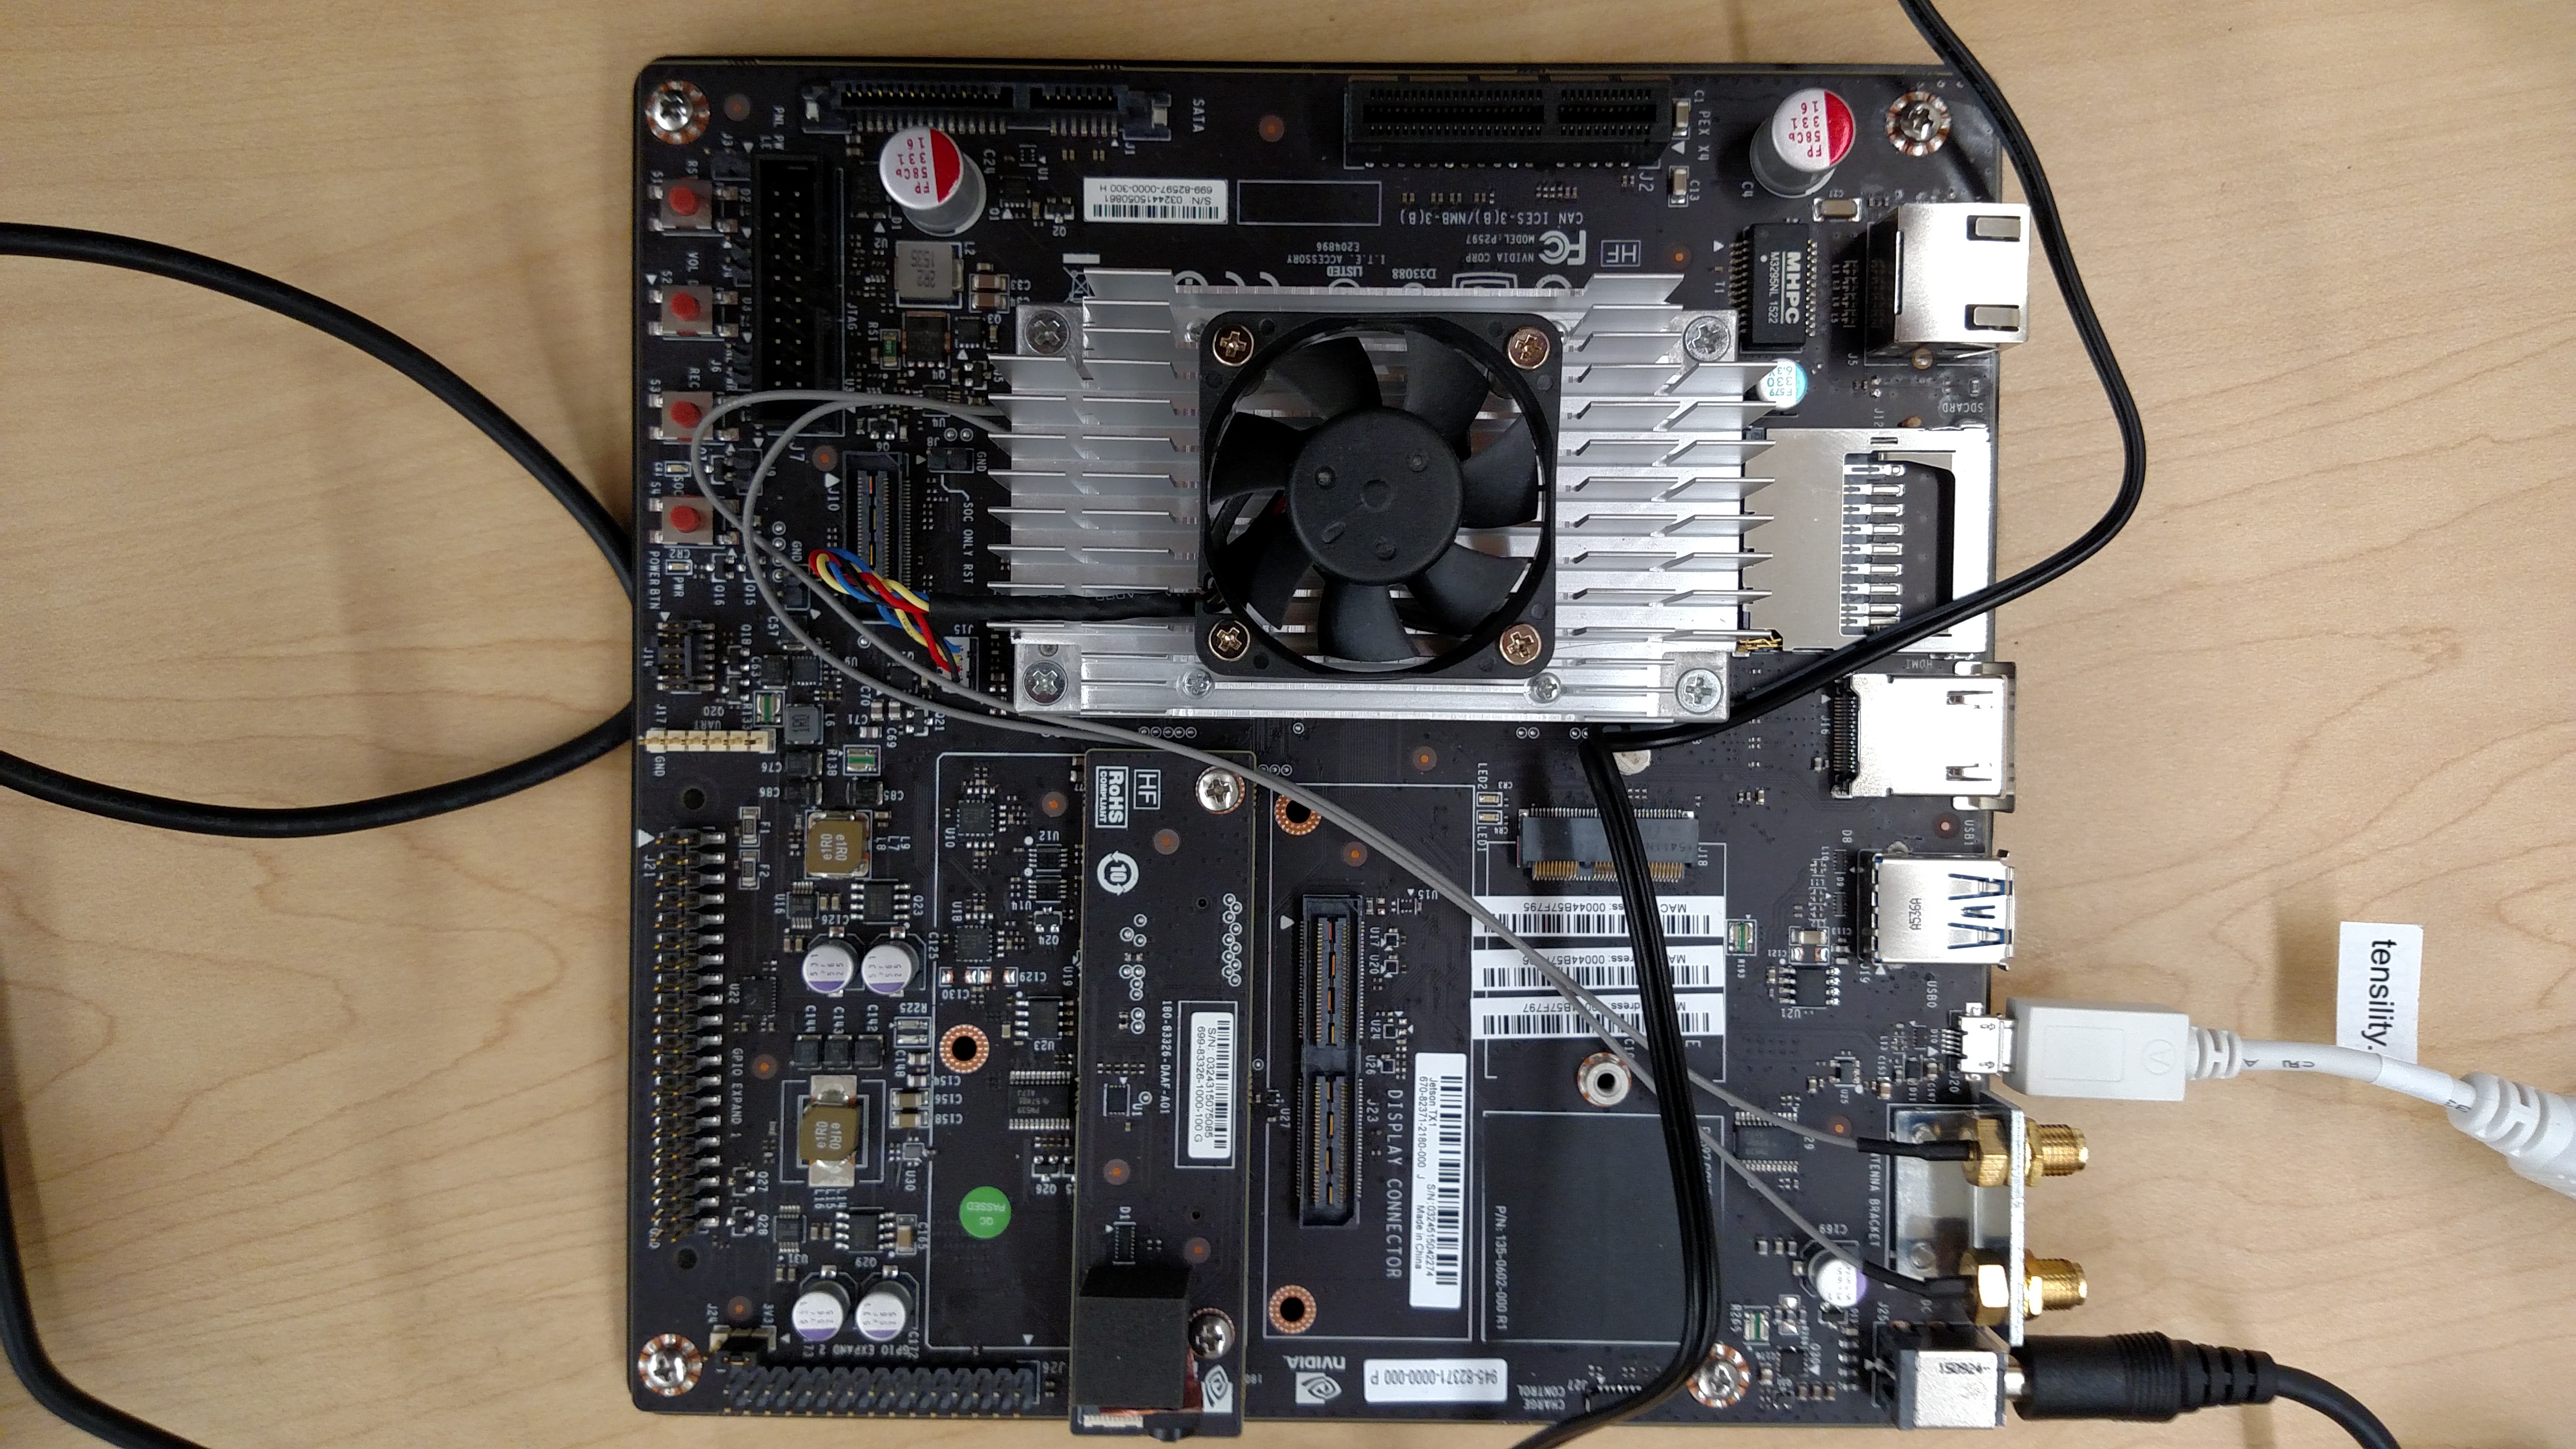
\includegraphics[width=0.6\textwidth,natwidth=610,natheight=642]{images/JetsonTX1.jpg}
		      \caption{The Jetson TX1}
				\end{figure}
\begin{figure}[!ht]
	  \centering
		    \includegraphics[width=0.6\textwidth,natwidth=610,natheight=642]{images/onboardCamera.JPG}
		     \caption{The on-board camera for the TX1}
				\end{figure}

\begin{figure}[!ht]
	  \centering
		    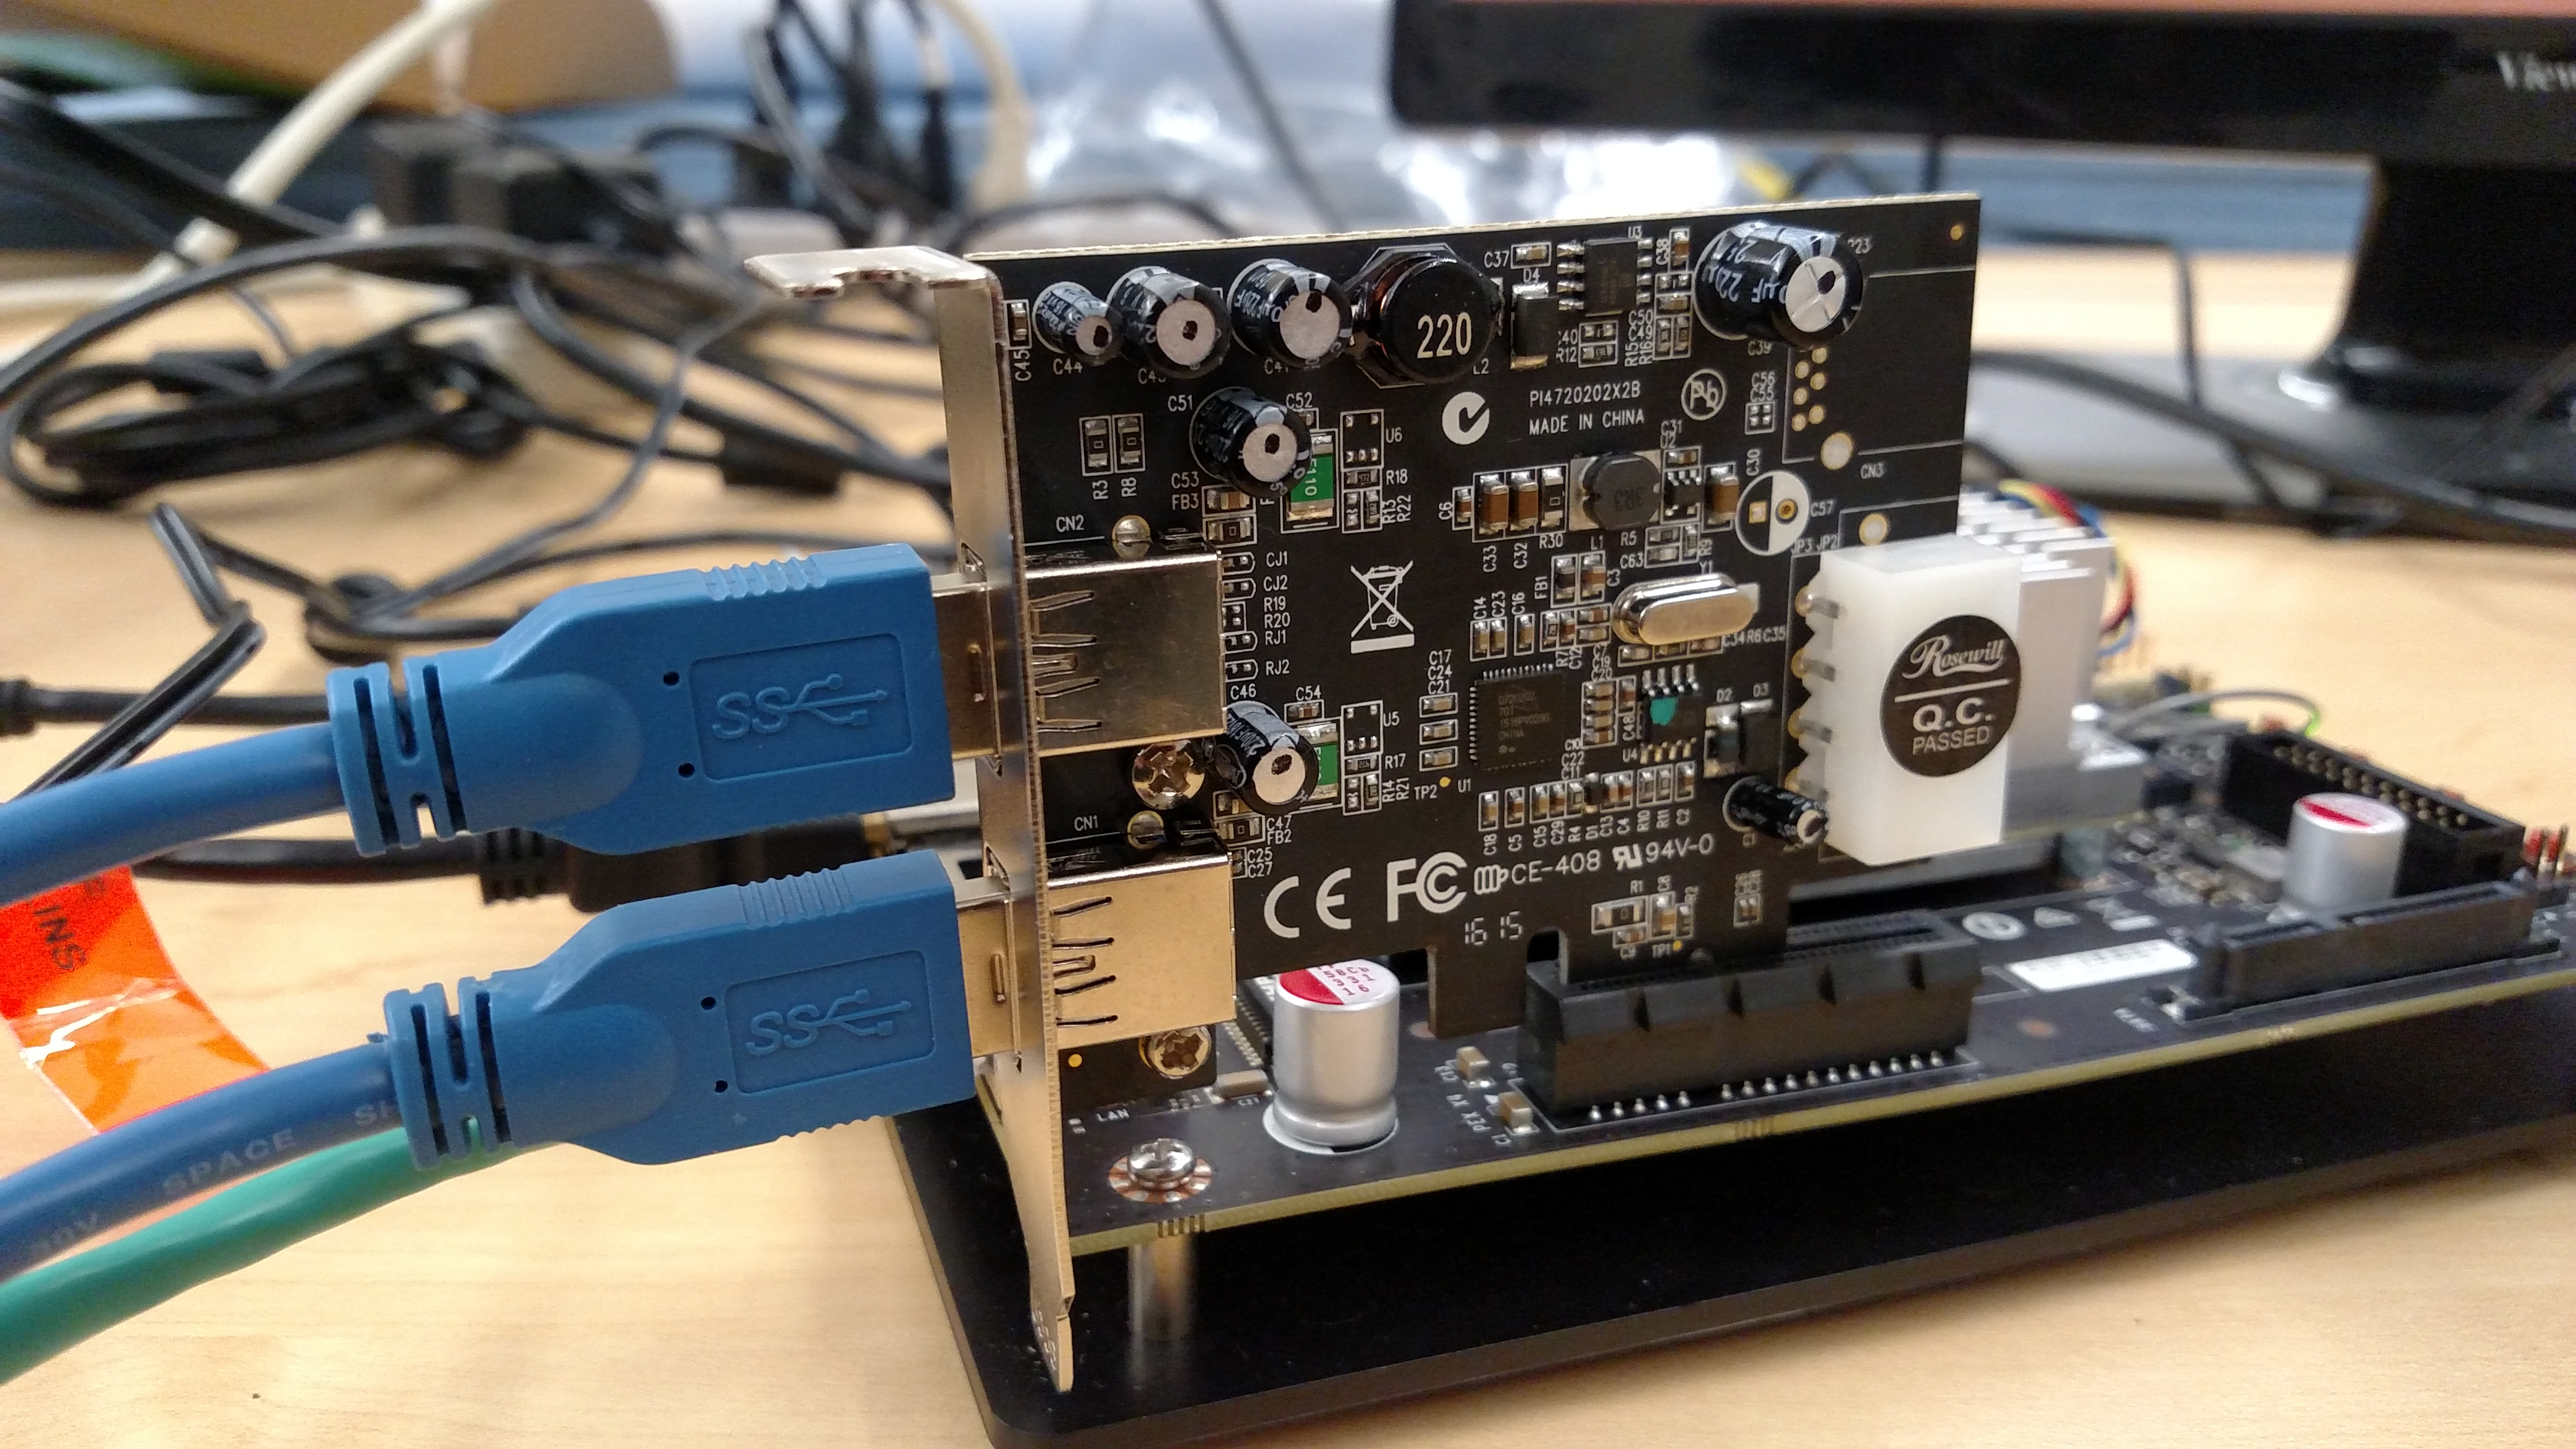
\includegraphics[width=0.6\textwidth,natwidth=610,natheight=642]{images/PCIe.jpg}
		      \caption{2-port USB 3.0 supersede PCIe Card}
				\end{figure}

\newpage
\subsection{Output Display Images}

Below are a few different images we were able to obtain with the use of our hardware and a few simple filters. Figure 6 and 7 are showing the original unprocessed output stream. Figure 6 is using the EVS-3000 lens and figure 7 is using the standard LS-TP-08 lens.\\

   \begin{figure}[!ht]
	  \centering
		    \includegraphics[width=0.6\textwidth]{images/normal_image.png}
		      \caption{Video output from the TX1 using a PointGrey camera with an EVS-3000 lens attached}
				\end{figure}
				
\begin{figure}[!ht]
	  \centering
		    \includegraphics[width=0.6\textwidth]{images/green_image.png}
		      \caption{Video output from the TX1 using a PointGrey camera with a LS-TP-08 lens attached}
				\end{figure}

\begin{figure}[!ht]
	  \centering
		    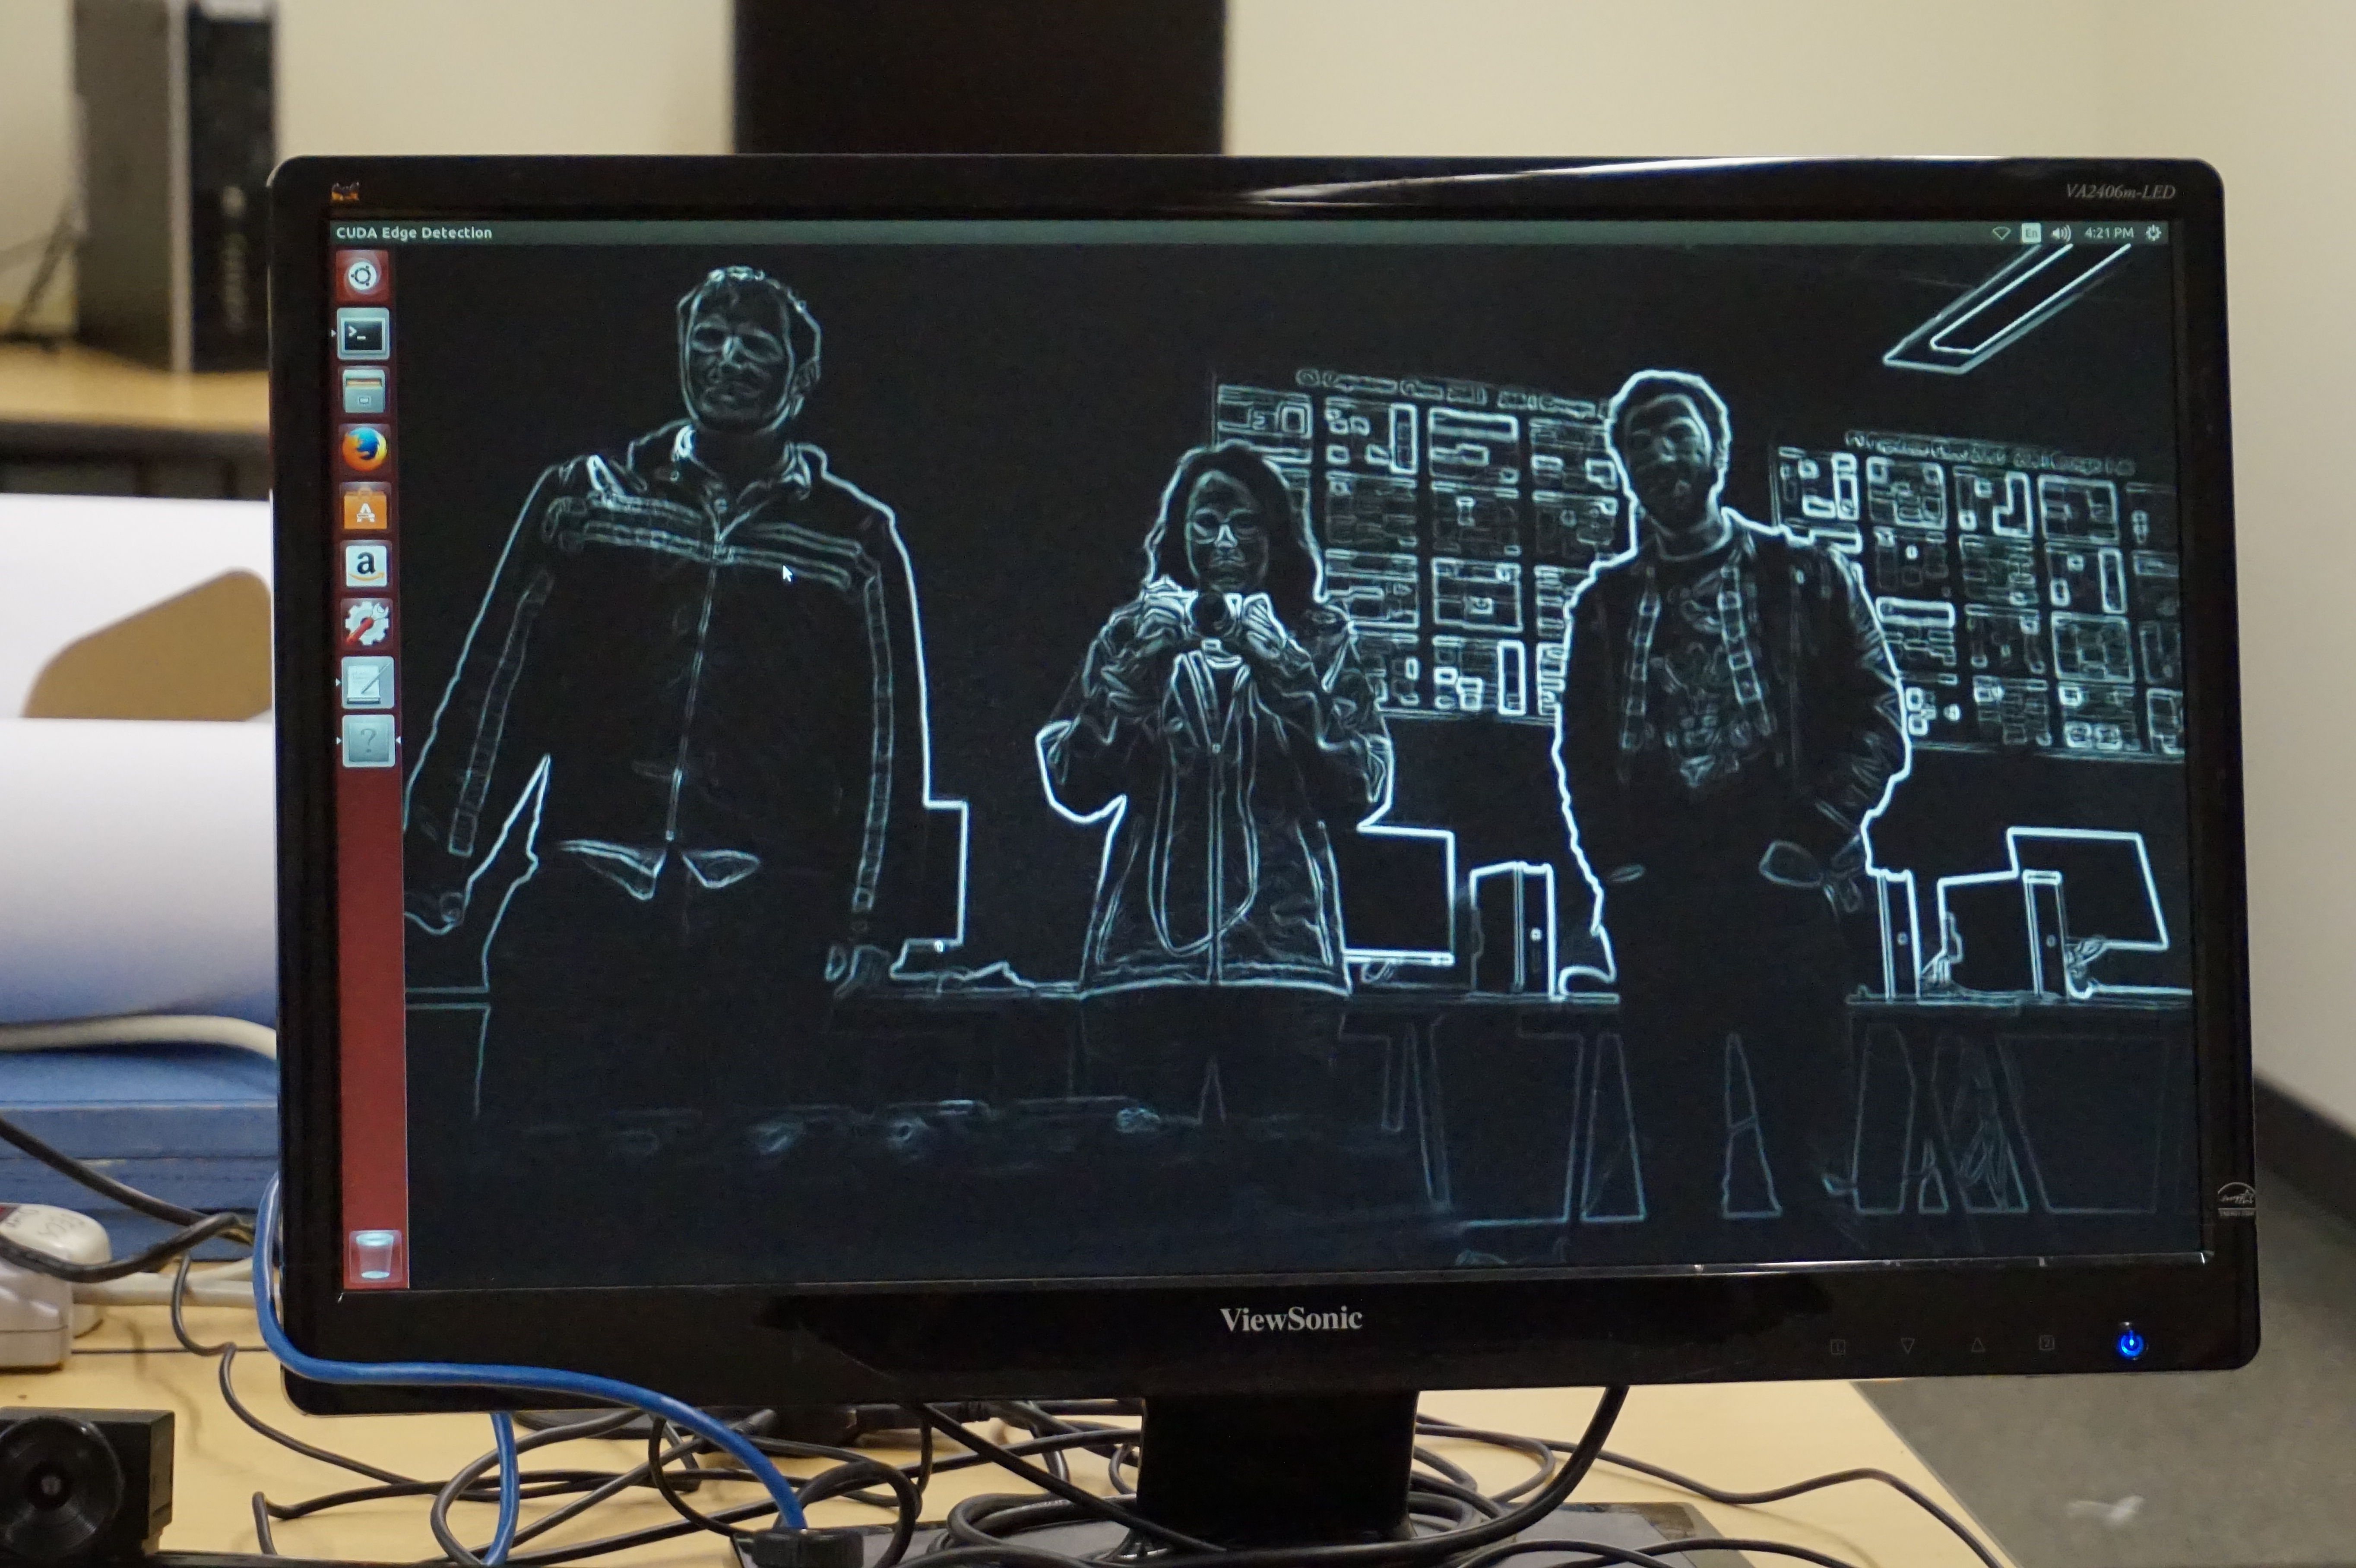
\includegraphics[width=0.6\textwidth]{images/line_detection.png}
		      \caption{Video output from the TX1 using a built-in OpenCV line detection filter}
				\end{figure}
 				
\begin{figure}[!ht]
	  \centering
		    \includegraphics[width=0.6\textwidth]{images/3_normal.png}
		      \caption{Video output from the TX1 overlaying three USB 3.0 video streams}
				\end{figure}
			
\begin{figure}[!ht]
\centering
\includegraphics[width=0.6\textwidth]{images/exampleOutputNormalBeta.jpg}
\caption{Video output from the TX1 running at ~85 fps}
\end{figure}